\documentclass[12pt]{article}
\usepackage{graphicx}
\usepackage[margin=0.8in]{geometry}
\begin{document}
{\bf Names:} Jack Bracewell, Milan Misak, Craig Ellis \\
{\bf Usernames:} jb2910, mm5510, ce710 \\
{\bf Group Number: 28}  \\ \\

\section*{Assignment 3: Artificial Neural Network}

\subsection*{Discuss how you obtained the optimal topology and optimal values of network parameters. Describe the performance measure you used (and explain why you preferred it over other measures) and the different topologies/parameters you experimented with.}

TODO \\


\subsection*{Explain what strategy you employed to ensure good generalisation ability of the networks and overcome the problem of overfitting.}

TODO \\


\subsection*{In Part VIII you used the optimal parameters that you found in part VI to train your networks. However, there is a problem with this approach, the data you used for validation at some point will be used for testing in cross-validation. Can you explain why this a problem? Ideally how should you optimise the parameters in cross-validation?}

TODO \\


\subsection*{Is there any difference in the classification performance of the two different classification approaches. Discuss the advantages/disadvantages of using 6 single-output NNs vs. 1 six-output NN.}

TODO: Is there any difference in classification performance? \\
\begin{itemize}
  \item The advantages of a six-output neural network are: the network will be weighted to give preference to one emotion over another, based on an attribute. For example, an attribute could indicate either emotion 1 or emotion 2 - separately, this gives us little information, but when evaluating both in the same network, perhaps the attribute is more likely to signify emotion 1 over emotion 2.
  \item The advantages of six single-output neural networks are: the networks are likely to be more TODO: accurate, since each one will weight its output focused purely on one emotion. This means weights, etc, will be specific to each tree - it will not be more general for all emotions, like in the multi-output tree.
\end{itemize}


\subsection*{Implementation details}
\begin{itemize}
  \item Cross-validation is done in much the same way as it was done for Decision Trees, with the exception that we needed two separate functions - one for the six one-output networks, and one for the six-output network. The cross-validation functions are passed the data received directly from ANNdata(), which is then split up in to training and validation data on each fold.
  \begin{itemize}
    \item For the six-output network, a network is created and trained using the optimal parameters we found, then used to predict the emotions of the validation inputs. These predictions are then compared to the correct outputs, and used to create the confusion matrix, etc
    \item The six one-output networks were similarly cross-validated, being represented by a cell-array of networks, which were easier to work with. The testANN() function, used to make the predictions, was modified to recognise whether or not the input was a cell-array, and to modify it accordingly, to make predictions (see below).
  \end{itemize}
  \item The outputs of the six one-output networks were combined in the testANN() function, into a single matrix like the one returned by the six-output network. this allowed the same function to be used for predictions (ie. the max value found for each column).
  \item TODO: anything else?
\end{itemize}


\subsection*{Evaluation results}

\subsubsection*{6-output network}

TODO

Something like:
Confusion matrix: The happiness tree was very good, perhaps overfit. Disgust and Happiness were quite often misclassified as well as correctly. They probably produced better trees because there was more data for them. Classification rate: The average classification rate is semi-successful as it succeeds most of the time. But it is far from perfect. Precision/Recall rate: The standout results are that sadness and fear are very difficult to identify correctly, most of the time they are not recognised. Wheras Hapiness was easy to recall but also registering many false positives. The anger tree was very cautious in making classifications but when it did, it was very successful.  F-measure: The F measures suggest as suspected that the Disgust and Happiness have well trained trees. Perhaps Sadness and Surprise did not have enough data. Anger is likely an easy emotion to classify given the trees high performance given a relatively small amount of data \\ \\

Confusion matrix: The happiness tree was very good, perhaps overfit. Disgust and Happiness were quite often misclassified as well as correctly. They probably produced better trees because there was more data for them. Classification rate: The average classification rate is semi-successful as it succeeds most of the time. But it is far from perfect. Precision/Recall rate:  F-measure: The F measures suggest as suspected that the Disgust and Happiness have well trained trees. Perhaps Sadness and Surprise did not have enough data. Anger is likely an easy emotion to classify given the trees high performance given a relatively small amount of data \\ \\


\subsubsection*{6 1-output networks}

TODO




\begin{table}
\centering
\begin{tabular}{r r | r r r r r r}
\multicolumn{8}{c}{Predicted class} \\
&  & Anger & Disgust & Fear & Happiness & Sadness & Surprise \\
\hline
& Anger & 7.4 & 1.4  & 0.4 & 2.0  & 0.9 & 1.1 \\
 & Disgust & 1.2 & 15.0 & 0   & 2.1  & 0.6 & 0.9 \\
Actual class & Fear & 0.5 & 2.3  & 3.9 & 1.8  & 0.8 & 2.6 \\
 & Happiness & 0.2 & 2.0  & 0   & 18.8 & 0.1 & 0.5 \\
& Sadness & 0.7 & 2.8  & 0.4 & 2.6  & 4.5 & 2.2 \\
& Surprise & 0   & 4.3  & 1.1 & 6.2  & 0.4 & 8.7 \\
\end{tabular}
\caption{Confusion matrix}
\end{table}

\begin{table}
\centering
\begin{tabular}{l | r r}
Emotion & Recall rate (\%) & Precision rate (\%) \\
\hline
Anger & 56.0606 & 74.0000 \\
Disgust & 75.7576 & 53.9568 \\
Fear & 32.7731 & 67.2414 \\
Happiness & 87.0370 & 56.1194 \\
Sadness & 34.0909 & 61.6438 \\
Surprise & 42.0290 & 54.3750 \\
\end{tabular}
\caption{Recall and precision rates}
\end{table}

\begin{table}
\centering
\begin{tabular}{l | r}
Emotion & \( F_1 \) measure \\
\hline
Anger & 63.7931 \\
Disgust & 63.0252 \\
Fear & 44.0678 \\
Happiness & 68.2396 \\
Sadness & 43.9024 \\
Surprise & 47.4114 \\
\end{tabular}
\caption{F1 measures}
\end{table}

Average classification rate = 0.5808 \\ 



\subsection*{Average performance per fold}

TODO


\subsection*{Code Flowchart}

TODO
%\begin{center}
%  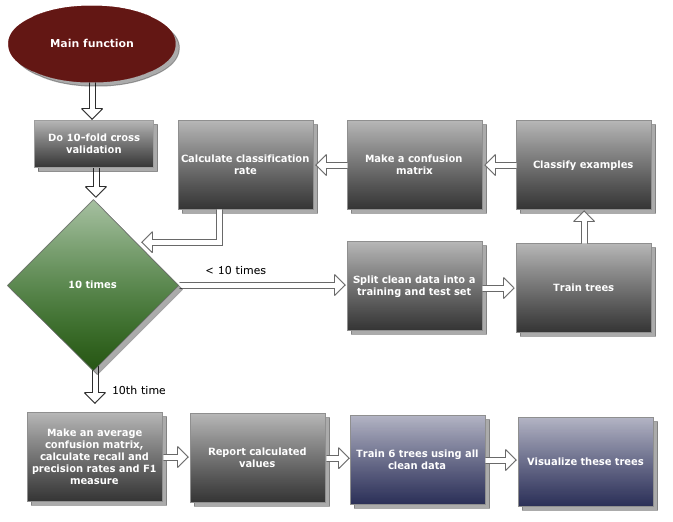
\includegraphics[scale=0.6]{report-images/flowchart.png}
%\end{center}

\end{document}
